%% Copernicus Publications Manuscript Preparation Template for LaTeX Submissions
%% ---------------------------------
%% This template should be used for copernicus.cls
%% The class file and some style files are bundled in the Copernicus Latex Package, which can be downloaded from the different journal webpages.
%% For further assistance please contact Copernicus Publications at: production@copernicus.org
%% https://publications.copernicus.org/for_authors/manuscript_preparation.html

%% copernicus_rticles_template (flag for rticles template detection - do not remove!)

%% Please use the following documentclass and journal abbreviations for discussion papers and final revised papers.

%% 2-column papers and discussion papers
\documentclass[soil, manuscript]{copernicus}



%% Journal abbreviations (please use the same for preprints and final revised papers)

% Advances in Geosciences (adgeo)
% Advances in Radio Science (ars)
% Advances in Science and Research (asr)
% Advances in Statistical Climatology, Meteorology and Oceanography (ascmo)
% Aerosol Research (ar)
% Annales Geophysicae (angeo)
% Archives Animal Breeding (aab)
% Atmospheric Chemistry and Physics (acp)
% Atmospheric Measurement Techniques (amt)
% Biogeosciences (bg)
% Climate of the Past (cp)
% DEUQUA Special Publications (deuquasp)
% Earth Surface Dynamics (esurf)
% Earth System Dynamics (esd)
% Earth System Science Data (essd)
% E&G Quaternary Science Journal (egqsj)
% EGUsphere (egusphere) | This is only for EGUsphere preprints submitted without relation to an EGU journal.
% European Journal of Mineralogy (ejm)
% Fossil Record (fr)
% Geochronology (gchron)
% Geographica Helvetica (gh)
% Geoscience Communication (gc)
% Geoscientific Instrumentation, Methods and Data Systems (gi)
% Geoscientific Model Development (gmd)
% History of Geo- and Space Sciences (hgss)
% Hydrology and Earth System Sciences (hess)
% Journal of Bone and Joint Infection (jbji)
% Journal of Micropalaeontology (jm)
% Journal of Sensors and Sensor Systems (jsss)
% Magnetic Resonance (mr)
% Mechanical Sciences (ms)
% Natural Hazards and Earth System Sciences (nhess)
% Nonlinear Processes in Geophysics (npg)
% Ocean Science (os)
% Polarforschung - Journal of the German Society for Polar Research (polf)
% Primate Biology (pb)
% Proceedings of the International Association of Hydrological Sciences (piahs)
% Safety of Nuclear Waste Disposal (sand)
% Scientific Drilling (sd)
% SOIL (soil)
% Solid Earth (se)
% State of the Planet (sp)
% The Cryosphere (tc)
% Weather and Climate Dynamics (wcd)
% Web Ecology (we)
% Wind Energy Science (wes)

% Pandoc citation processing

% The "Technical instructions for LaTex" by Copernicus require _not_ to insert any additional packages.
% % % From pandoc table feature
% \usepackage{longtable,booktabs,array}
% % \usepackage{calc} % for calculating minipage widths
% % Correct order of tables after \paragraph or \subparagraph
% \usepackage{etoolbox}
% \makeatletter
% \patchcmd\longtable{\par}{\if@noskipsec\mbox{}\fi\par}{}{}
% \makeatother
% % Allow footnotes in longtable head/foot
% \IfFileExists{footnotehyper.sty}{\usepackage{footnotehyper}}{\usepackage{footnote}}
% \makesavenoteenv{longtable}
% 
% tightlist command for lists without linebreak
\providecommand{\tightlist}{%
  \setlength{\itemsep}{0pt}\setlength{\parskip}{0pt}}


%
%% \usepackage commands included in the copernicus.cls:
%\usepackage[german, english]{babel}
%\usepackage{tabularx}
%\usepackage{cancel}
%\usepackage{multirow}
%\usepackage{supertabular}
%\usepackage{algorithmic}
%\usepackage{algorithm}
%\usepackage{amsthm}
%\usepackage{float}
%\usepackage{subfig}
%\usepackage{rotating}

\begin{document}


\title{Wall-to-wall mapping of peat depth from Lidar terrain and airborne radiometrics in Norwegian landscapes}


\Author[1][julien.vollering@hvl.no]{Julien}{Vollering}
\Author[2]{Naomi}{Gatis}
\Author[1]{Mette}{Kusk Gillespie}
\Author[1]{Karl-Kristian}{Muggerud}
\Author[1]{Sigurd Daniel}{Nerhus}
\Author[1]{Knut}{Rydgren}
\Author[1]{Mikko}{Sparf}


\affil[1]{Department of Civil Engineering and Environmental Sciences, Western Norway University of Applied Sciences, Norway}
\affil[2]{Department of Geography, University of Exeter, United Kingdom}

\runningtitle{Peat depth from terrain and radiometrics}

\runningauthor{Vollering et al.}


\correspondence{Julien\ Vollering\ (julien.vollering@hvl.no)}



\received{}
\pubdiscuss{} %% only important for two-stage journals
\revised{}
\accepted{}
\published{}

%% These dates will be inserted by Copernicus Publications during the typesetting process.


\firstpage{1}

\maketitle


\begin{abstract}
The abstract goes here.
It can also be on \emph{multiple lines}.
\end{abstract}




\section{Introduction}

Introduction text goes here.
Read Gatis et al. \citeyearpar{gatisMappingUplandPeat2019} and related work \citep{minasnyDigitalMappingPeatlands2019}.

\section{Materials and methods}

\subsection{Sites}

We assessed how well we could predict peat depth at two sites with conspicuously different physical geography: Skrimfjella in eastern Norway and Ørskogfjellet in western Norway (Fig. \ref{fig:sites}c).
These sites were chosen because they were covered by radiometric data from airborne surveys, relatively little built-up area, and road access.

\begin{figure}
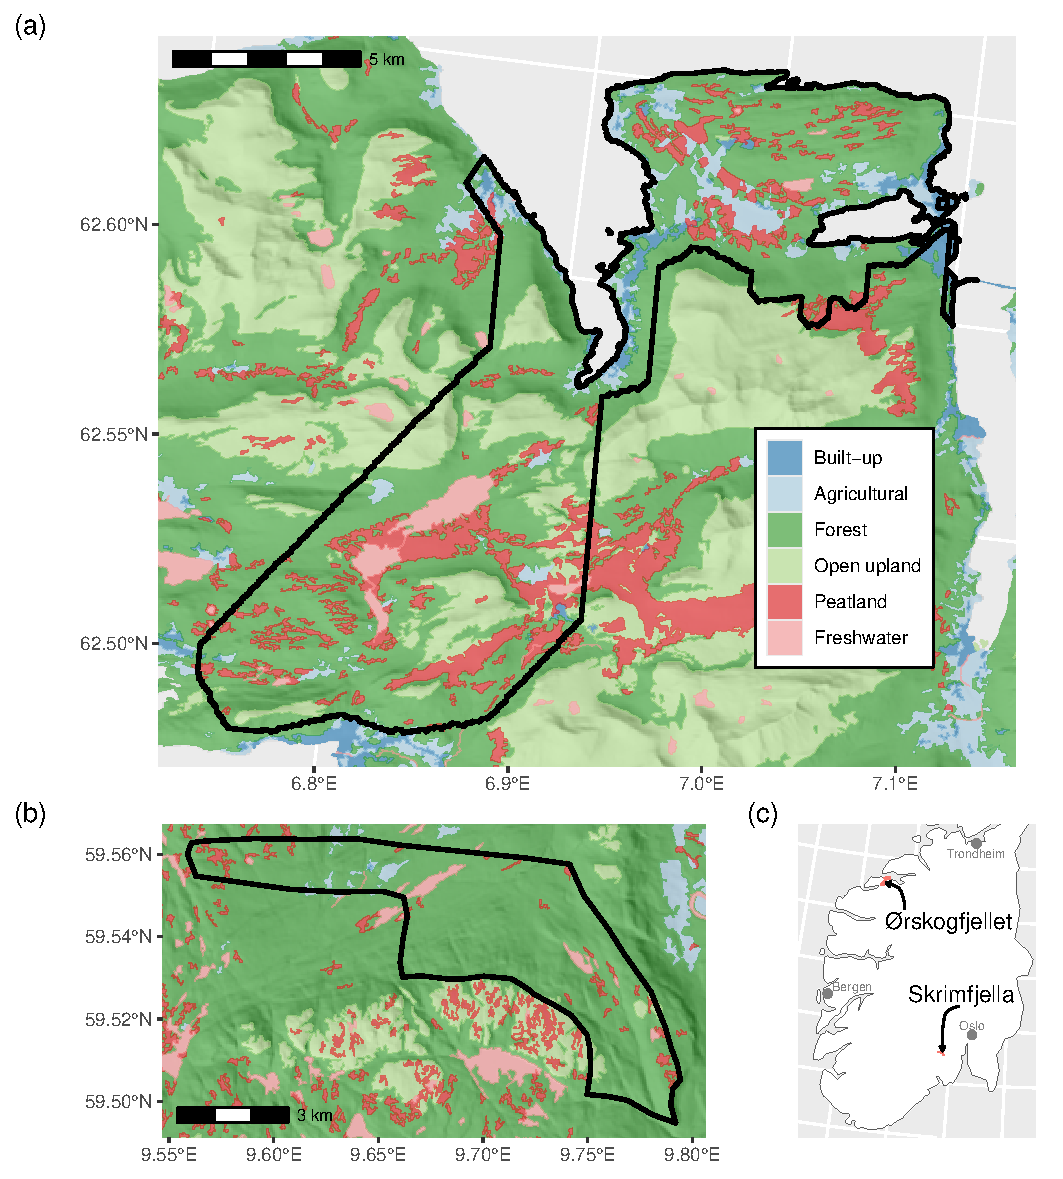
\includegraphics[height=0.9\textheight]{figures/sites-patchwork} \caption{Study areas at Ørskogfjellet (a) and Skrimfjella (b) within southern Norway (c). Land cover shown here is from the AR50 national land resource database and has simplified geometry with respect to the AR5 database used in the study.}\label{fig:sites}
\end{figure}

At Skrimfjella we delineated a study area of \unit{34\,km^{2}} based on radiometric coverage and accessibility (Fig. \ref{fig:sites}b).\\
The landscape within our delineation is classified as \emph{inland hills and mountains} \citep{simensenDiversityDistributionLandscape2021}.
It is almost without human infrastructure, dominated by forest, and borders on a large nature reserve.
The study area has a mean elevation of \unit{438\,m} above sea level (range 223--711, IQR 351--509), and its mean slope at \unit{10\,m} resolution is 10.8° (IQR 4.6--15.1°).
In Norway's AR5 national land capability dataset \citep{ahlstromAR5Klassifikasjonssystem2019}, \unit{1.5\,km^{2}} (4.5 \%) of the study area is classified as mire --- defined as areas with mire vegetation and at least \unit{30\,cm} of peat depth.

At Ørskogfjellet we defined a study area of \unit{124\,km^{2}} which basically followed the footprint of the radiometric survey (Fig. \ref{fig:sites}a).
This study area comprises a wide range of major landscape types: \emph{coastal plains}, \emph{coastal fjord}, \emph{inland valleys}, as well as \emph{inland hills and mountains} \citep{simensenDiversityDistributionLandscape2021}.
It is mostly forested, but also contains considerable farmland and open upland, and has several large lakes.
Its mean elevation is \unit{211\,m} above sea level (range 0--807, IQR 73--310), and its mean slope at \unit{10\,m} resolution is 13.0° (IQR 4.7--18.3°).
The AR5 dataset counts \unit{15.3\,km^{2}} (12.4 \%) of the study area as mire.

\subsection{Peat depth measurements}

At both study sites, our measurements of peat depth were made for the purpose of training a machine learning model of peat depth, and we designed our sampling with this in mind \citep{brusSamplingDigitalSoil2019}.
Broadly, we aimed for a sample that was representative the predictor space of the most important predictors of peat depth \citep{wadouxSamplingDesignOptimization2019, maComparisonConditionedLatin2020}.
A sample that preserves the properties of the multivariate distribution of predictor and outcome variables is most likely to maintain any complex, non-linear relationships that exist in the population while avoiding spurious ones \citep{brusSamplingDigitalSoil2019}.
We chose for our sampling and modelling a spatial resolution of \unit{10\,m}.
We considered this a reasonable compromise between digital terrain model resolution (\unit{1\,m}) and small mires on the one hand, and airborne radiometric resolution (\unit{50\,m}) on the other.

\subsubsection{Skrimfjella}

We measured peat depth in selected locations (\unit{10\,m} raster cells) at Skrimfjella.
The locations were chosen only from areas delineated as mire in the AR5 national land capability dataset.
Within this mire area, we stratified our sample across values of elevation, slope, and potassium ground concentration \citep[from processed airborne gamma ray spectrometry,][]{baranwalHelicopterborneMagneticElectromagnetic2013}.
Specifically, we used the \emph{eSample} function in the \emph{iSDM} R package (v.1.0) to chose an environmentally systematic sample.
This function defines the environmental space as a two-dimensional convex hull around the ordinated data, then creates a regular grid across that space, and lastly finds for each grid cell the datum that is nearest \citep{hattabUnifiedFrameworkModel2017}.
Elevation was extracted from the \unit{10\,m} national digital terrain model, slope calculated in degrees, and potassium ground concentration downscaled with bilinear resampling.
We set a target sample size of 100, excluded the top and bottom percentile from the convex hull, and with these parameters \emph{eSample} returned 105 raster cells.

In addition to the peat depth locations, we had another arm of our sampling design for measuring peatland occurrence, as binary variable.
We wanted to measure peatland occurrence outside of mapped mire areas because the AR5 dataset is known to underestimate peatland coverage \citep[especially in forests,][]{brynLandCoverNorway2018}, and because airborne radiometrics may help identify unmapped peatland \citep{gatisMappingUplandPeat2019, olearyDigitalSoilMapping2022}.
The occurrence locations were sampled from the part of the study area that (1) was mapped as something other than mire in the AR5 database and (2) had a slope \textless{} 20°.
We performed environmentally systematic sampling of this population with the same procedure as for the depth locations, and \emph{eSample} returned 106 raster cells.

Field work at Skrimfjella was conducted in August 2020.
We navigated to the centers of the raster cells in the depth and occurrence samples by handheld GPS, checking that positional error was below \unit{3\,m}.
For each depth sample location, we measured peat depth three times (at the vertices of a triangle with \unit{2\,m} sides) to get a more representative value for the \unit{10\,m} raster cell, and to dampen the effect of outlying measurements \citep{parryEvaluatingApproachesEstimating2014}.
We used a metal probe pushed downward until resistance indicated the base of the peat column.
Probe locations were adjusted up to \unit{20\,cm} if the base of the peat column seemed to be blocked by an obvious artifact.
For each occurrence sample location, we recorded the presence or absence of peatland --- primarily by digging and examining the top \unit{20\,cm} of soil (where this was possible).
We judged whether the soil was a peat soil based on its density, texture, and color.
Occasionally, when the soil itself was difficult to judge, we made our determination also based on the presence or absence of mire vegetation.
Although peat soil is strictly defined by organic content (which we did not analyse), we believe our protocol produced reasonable determinations of presence or absence that would generally satisfy most of the varying definitions of peatland \citep{minasnyMappingMonitoringPeatland2023}.

Besides the depth and occurrence measurements described above, we also measured peat depth in three subjectively-chosen, individual mires, using ground-penetrating radar (GPR).
We used the Malå ProEx GPR system (Guideline Geo AB, Sweden) with its \unit{500\,MHz} shielded antenna mounted in a plastic sledge, and its control unit connected to a GNSS receiver.
At each of the three mires we recorded GPR traces along walking transects that covered the extent of the mire, mostly in traversing, zigzag patterns with between \unit{5\,m} and \unit{20\,m} spacing at their vertices.
Along the GPR transects we also probed peat depth at marked trace locations, to be able to calibrate the GPR wave speed velocity.
We processed the GPR data with Reflex2DQuick software (v.3.0; Sandmeier Scientific Software, Germany), applying a time-zero correction, a dewow filter, and a gain filter based on observed energy decay.
Then we picked strong reflectors in the radargrams that we interpreted as the base of the peat column.
We used picks at marked trace locations to calibrate wave speed velocity; we pooled calibration points across the three mires and fitted a linear regression of depth on one-way travel time with the intercept fixed at zero.
In total we had 46 calibration points along \unit{3.5\,km} of GPR transects.
Finally, we used the calculated wave velocity (\unit{0.0387\,m\,ns^{-1}}, \(R^2 = 0.874\)) to convert the travel times of all picks to calibrated peat depths.

\subsubsection{Ørskogfjellet}

Subsubsection text here.

\subsection{Peat depth predictors}

\subsection{Predictive models of peat depth}

\section{Results}

Include a 12cm width figure of Nikolaus Copernicus from \href{https://en.wikipedia.org/wiki/File:Nikolaus_Kopernikus.jpg}{Wikipedia} with caption using R Markdown (Fig. \ref{fig:portrait}).

\begin{figure}
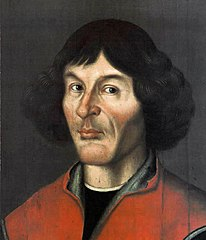
\includegraphics[width=8.3cm]{Nikolaus_Kopernikus} \caption{one column figure}\label{fig:portrait}
\end{figure}

\subsection{Tables}

You can add \LaTeX table in an R Markdown document to meet the template requirements (Table \ref{tab:latextable}).

\begin{table}[t]
\caption{TEXT}
\begin{tabular}{l c r}
\tophline

a & b & c \\
\middlehline
1 & 2 & 3 \\

\bottomhline
\end{tabular}
\belowtable{Table Footnotes}
\label{tab:latextable}
\end{table}

Or you can use markdown to create the table with booktabs = FALSE (\url{https://github.com/rstudio/rticles/issues/558\#issuecomment-1907981541}).

See Table \ref{tab:test}.

\begin{table}

\caption{\label{tab:test}My caption}
\centering
\begin{tabular}[t]{l|r|r|r}
\hline
  & mpg & cyl & disp\\
\hline
Mazda RX4 & 21.0 & 6 & 160\\
\hline
Mazda RX4 Wag & 21.0 & 6 & 160\\
\hline
Datsun 710 & 22.8 & 4 & 108\\
\hline
\end{tabular}
\end{table}

\section{Discussion}

Lorem ipsum dolor sit amet, consectetur adipiscing elit.
Sed do eiusmod tempor incididunt ut labore et dolore magna aliqua.
Ut enim ad minim veniam, quis nostrud exercitation ullamco laboris nisi ut aliquip ex ea commodo consequat.
Duis aute irure dolor in reprehenderit in voluptate velit esse cillum dolore eu fugiat nulla pariatur.
Excepteur sint occaecat cupidatat non proident,
sunt in culpa qui officia deserunt mollit anim id est laborum.

\section{Conclusions}

Nulla facilisi.
Maecenas vel nunc nec purus tincidunt congue.
Proin auctor, lectus eu pharetra malesuada,
nisi nunc bibendum nunc,
eget tincidunt nunc nisi id nunc.
Sed euismod, nunc sit amet aliquam tincidunt,
nunc nunc tincidunt nunc,
nec tincidunt nunc nunc nec nunc.
Donec auctor, nunc sit amet aliquam tincidunt,
nunc nunc tincidunt nunc,
nec tincidunt nunc nunc nec nunc.



\codedataavailability{\emph{Code and data availability.} Use this to add a statement when having data sets and software code available} %% use this section when having data sets and software code available



%%%%%%%%%%%%%%%%%%%%%%%%%%%%%%%%%%%%%%%%%%
%% optional

%%%%%%%%%%%%%%%%%%%%%%%%%%%%%%%%%%%%%%%%%%
\appendix
\section{For submission}

``Appendices: all material required to understand the essential aspects of the paper
such as experimental methods, data, and interpretation
should preferably be included in the main text.
Additional figures, tables, as well as technical and theoretical developments
which are not critical to support the conclusion of the paper,
but which provide extra detail and/or support useful for experts in the field
and whose inclusion in the main text would disrupt the flow of descriptions or demonstrations
may be presented as appendices.
These should be labelled with capital letters: Appendix A, Appendix B etc.
Equations, figures and tables should be numbered as (A1), Fig. B5 or Table C6, respectively.
Please keep in mind that appendices are part of the manuscript
whereas supplements (see below) are published along with the manuscript.''

\section{Figures and tables in appendices}

Please also sort the appendix figures and appendix tables into the respective appendix sections.
They will be correctly named automatically.

\section{Copernicus from Rmarkdown}

\textbf{Please note:} Per \href{https://publications.copernicus.org/for_authors/manuscript_preparation.html}{their guidelines},
Copernicus does not support additional \LaTeX{} packages
or new \LaTeX{} commands than those defined in their \texttt{.cls} file.
This means that you cannot add any extra dependencies
and a warning will be thrown if so.
\textbf{Important}: Always double-check with the official manuscript preparation guidelines
at \url{https://publications.copernicus.org/for_authors/manuscript_preparation.html},
especially the sections ``Technical instructions for LaTeX'' and ``Manuscript composition''.
Please contact Daniel Nüst, \texttt{daniel.nuest@uni-muenster.de}, with any problems.
\noappendix

%%%%%%%%%%%%%%%%%%%%%%%%%%%%%%%%%%%%%%%%%%
\authorcontribution{\emph{Author contributions.}
JV: Conceptualization, Investigation, Data curation, Formal analysis, Writing -- original draft.
NG: Conceptualization, Methodology, Writing - review \& editing.
MKG: Investigation, Writing - review \& editing.
KKM: Investigation, Data curation, Writing - review \& editing.
SDN: Investigation, Writing - review \& editing.
KR: Conceptualization, Investigation, Writing - review \& editing.
MS: Investigation, Data curation, Writing - review \& editing.} %% optional section

%%%%%%%%%%%%%%%%%%%%%%%%%%%%%%%%%%%%%%%%%%
\competinginterests{\emph{Competing interests.} The authors declare that they have no conflict of interest.} %% this section is mandatory even if you declare that no competing interests are present

%%%%%%%%%%%%%%%%%%%%%%%%%%%%%%%%%%%%%%%%%%
\disclaimer{\emph{Disclaimer.} The authors declare that the results, discussions, and interpretations presented in this study are solely their own. The views expressed herein do not necessarily reflect those of their respective institutions or funding agencies.} %% optional section

%%%%%%%%%%%%%%%%%%%%%%%%%%%%%%%%%%%%%%%%%%
\begin{acknowledgements}
\emph{Acknowledgements.} We thank the Norwegian Public Roads Administration for sharing data from ground-penetrating radar surveys. We also thank Vikas Baranwal from the Geological Survey of Norway for helping us access the radiometric data from Skrim.
\end{acknowledgements}

%% REFERENCES
%% DN: pre-configured to BibTeX for rticles

%% The reference list is compiled as follows:
%%
%% \begin{thebibliography}{}
%%
%% \bibitem[AUTHOR(YEAR)]{LABEL1}
%% REFERENCE 1
%%
%% \bibitem[AUTHOR(YEAR)]{LABEL2}
%% REFERENCE 2
%%
%% \end{thebibliography}

%% Since the Copernicus LaTeX package includes the BibTeX style file copernicus.bst,
%% authors experienced with BibTeX only have to include the following two lines:
%%
\bibliographystyle{copernicus}
\bibliography{ms.bib}
%%
%% URLs and DOIs can be entered in your BibTeX file as:
%%
%% URL = {http://www.xyz.org/~jones/idx_g.htm}
%% DOI = {10.5194/xyz}


%% LITERATURE CITATIONS
%%
%% command                        & example result
%% \citet{jones90}|               & Jones et al. (1990)
%% \citep{jones90}|               & (Jones et al., 1990)
%% \citep{jones90,jones93}|       & (Jones et al., 1990, 1993)
%% \citep[p.~32]{jones90}|        & (Jones et al., 1990, p.~32)
%% \citep[e.g.,][]{jones90}|      & (e.g., Jones et al., 1990)
%% \citep[e.g.,][p.~32]{jones90}| & (e.g., Jones et al., 1990, p.~32)
%% \citeauthor{jones90}|          & Jones et al.
%% \citeyear{jones90}|            & 1990


\end{document}
